\begin{figure*}[t!]
    \centering
    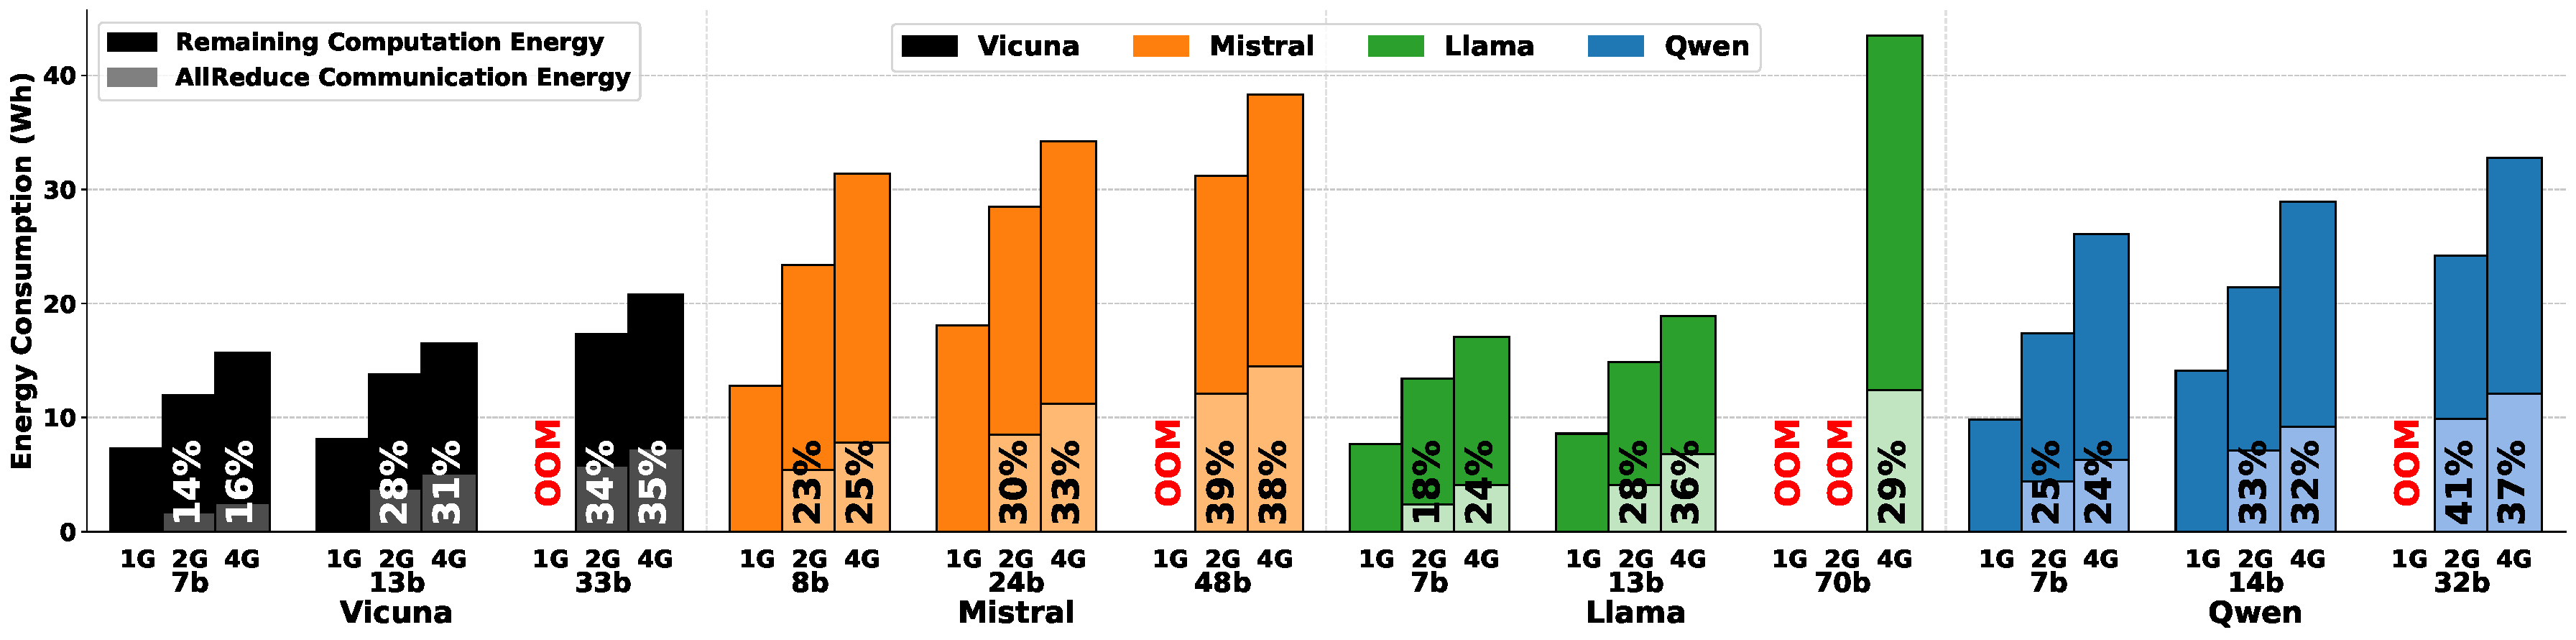
\includegraphics[width=\textwidth]{figures/llm_energy_comparison.pdf}
    \vspace{-24pt}
    \caption{Energy consumption across models and GPU configurations (2- and 4-GPU runs use tensor parallelism). Bars show total model energy; lighter segments show AllReduce communication energy (\% shown) and darker segments show remaining computation energy. Missing bars denote cases where model did not fit in GPU memory.} 
    \vspace{-15pt}
    \label{fig:all_reduce_energy}
\end{figure*}

%Our goal is to develop a methodology for predicting the energy consumption of parallel LLM inference over multiple GPUs.
There are three main parallelism strategies that are widely used for LLM inference, described below in increasing order of complexity.
%%%(see Appendices~\ref{app:collective-background} and \ref{app:data-collection-parallel} for more details).
\begin{enumerate}[leftmargin=*,itemsep=0pt,topsep=0pt]
    \item \textbf{Data parallelism} replicates the entire LLM on multiple GPUs, allowing input data to be processed in parallel~\cite{data-parallel}.
    \item \textbf{Pipeline parallelism} partitions the LLM into $s$ sequential stages, assigning each stage to a different GPU and processing micro-batches in a pipeline~\cite{sangjin23_envpipe}. 
    \item \textbf{Tensor parallelism} splits individual model computations (such as matrix multiplications) across multiple GPUs to enable parallel execution of operations~\cite{megatron}.
\end{enumerate}

\review{Tensor, pipeline, and data parallelism expose distinct communication patterns. In tensor parallelism, GPUs jointly execute operations within a layer, so partial results must be exchanged and combined using collectives such as AllReduce. Because these collectives occur repeatedly throughout the forward pass, communication is closely coupled with computation and synchronization.}

\review{Pipeline parallelism partitions layers across stages, and each stage sends its output activations to the next stage using point-to-point communication. Communication therefore occurs primarily at stage boundaries as activations move through the pipeline.}

\review{In data parallelism, each replica independently executes the full model on a different portion of the workload. Communication is therefore limited during the forward computation, with collective operations such as AllGather used when outputs from multiple replicas need to be consolidated.}

%Our framework can be extended to other strategies such as hybrid parallelism that combines existing parallelism methods; we leave this to future work.
%\medskip
%\subsection*{Challenges in predicting parallel inference energy}

There are two key challenges in accurately predicting the energy of parallel inference strategies.

\noindent\textbf{Compute energy.}
Even in single-GPU inference, compute energy depends on how \emph{each module}'s operator mix maps to GPU execution (e.g., memory behavior), which varies with tensor shapes and hardware/resource characteristics. 
%The energy traces for 10,000 individual Vicuna inference runs, collected on a NVIDIA A6000 GPU, are visibly noisy as well, as seen in(Figure~\ref{fig:energy-variance}).
%\anshul{need more details about the experiment, like which model and maybe point to S5x for experimental setup details. also, this figure should maybe go in non-determinism para, like the last para in this section?}
%\anurag{This is a single-GPU experiment, putting it in communication section seems improper as there is no communication here.}
%As a result, accurate modeling requires \emph{module-level} predictors that condition on both architecture-derived and resource/runtime features rather than a single aggregate utilization signal. 
In multi-GPU inference, this is further complicated because each module's computation and data may be divided across GPUs, so the model has to account for the energy consumption of the module at each GPU.
%%module computation is \be{sharded} across devices, so predicting a module's compute energy requires accounting for the per-rank shard (its local tensor shapes and execution) and then composing these shard-level estimates into an end-to-end module-level energy estimate. \aruna{I dont think I quite understand what this challenge is and how we solve it}

% Even in single-GPU inference, compute energy is difficult to predict because it is not a simple analytical function of token counts or average utilization. Instead, it depends on how the model’s operator mix maps to GPU execution at a fine granularity: different layers alternate between compute- and memory-bound phases, exhibit different cache reuse and memory-traffic patterns, and trigger different kernel schedules and concurrency across SMs.
% These effects make energy sensitive to seemingly small changes in tensor shapes (e.g., batch size, prefill vs.\ decode, and sequence-length-dependent activation sizes), and to runtime dynamics such as kernel launch ordering and power-state behavior under bursty workloads.
% In multi-GPU inference, these compute-side sensitivities persist on each GPU, but become more consequential because small per-GPU compute fluctuations can create \emph{stragglers} that change when synchronization points are reached, thereby affecting end-to-end energy beyond the local compute cost.
% \anurag{Make the compute energy smaller}

\noindent\textbf{Communication energy.}
\review{Multi-GPU inference additionally incurs \emph{substantial} energy from inter-GPU communication, including AllReduce in tensor parallelism, point-to-point transfers in pipeline parallelism, and AllGather in data parallelism, which is absent in single-device execution.}
% \noindent\textbf{Communication energy.}
% Multi-GPU inference additionally incurs \emph{substantial} energy from inter-GPU communication (e.g., AllReduce/ReduceScatter/AllGather, see Appendix~\ref{app:collective-background}), 
%\aruna{if you define these somewhere in the appendix, please add a reference}, 
% which is absent in single-device execution.
%and can form a large fraction of end-to-end energy. 
Figure~\ref{fig:all_reduce_energy} shows the measured energy consumption for 4 different LLM models under different GPU settings;
%(some larger models run out of memory when run with limited parallelization). 
details of the setup can be found in \S\ref{s:evaluation}. 
 Communication energy accounts for a large fraction (up to 41\%) of the total energy consumption.
%is due to communication energy, denoted as lighter segments in the figure.
% \be{Predicting communication energy is challenging} because communication is not a standalone phase: in tensor parallelism, collectives are frequently \emph{interleaved with} and \emph{overlapped with} computation for efficiency, so the measured energy reflects a mixture of compute, data movement, and synchronization overhead.
%%As such, communication modules must be \emph{accounted for explicitly} in the model tree; ignoring them leads to large prediction errors (see \S\ref{sec:ablation}).
%Accurately measuring this component is challenging as it requires tracking each of the numerous communication events on each GPU.
Tensor parallelism specifically introduces additional variance in energy consumption as
GPUs may lag/lead each other non-deterministically.
%but because they have to synchronize with each other frequently, the total energy consumption is non-deterministic. 

%This introduces additional complications due \be{synchronization induced non-determinism} %that directly perturbs communication energy across runs.
%collective-related GPU/NIC buffer activity begins and when transfer completes across the cluster, and then benchmarking these collectives under the target GPU count and topology to obtain representative energy costs that can be composed with module-level compute predictions.
% \anurag{I am sure we definitely do this and the design section will reflect this}
%\arunacomment{This last sentence sounds complicated and it is not clear to me how we are addressing this.}
%\anshul{I simplified the last sentence a bit, check. this says why direct measurement of comm energy is challenging}
%\begin{figure}[t]
    % \centering
 %   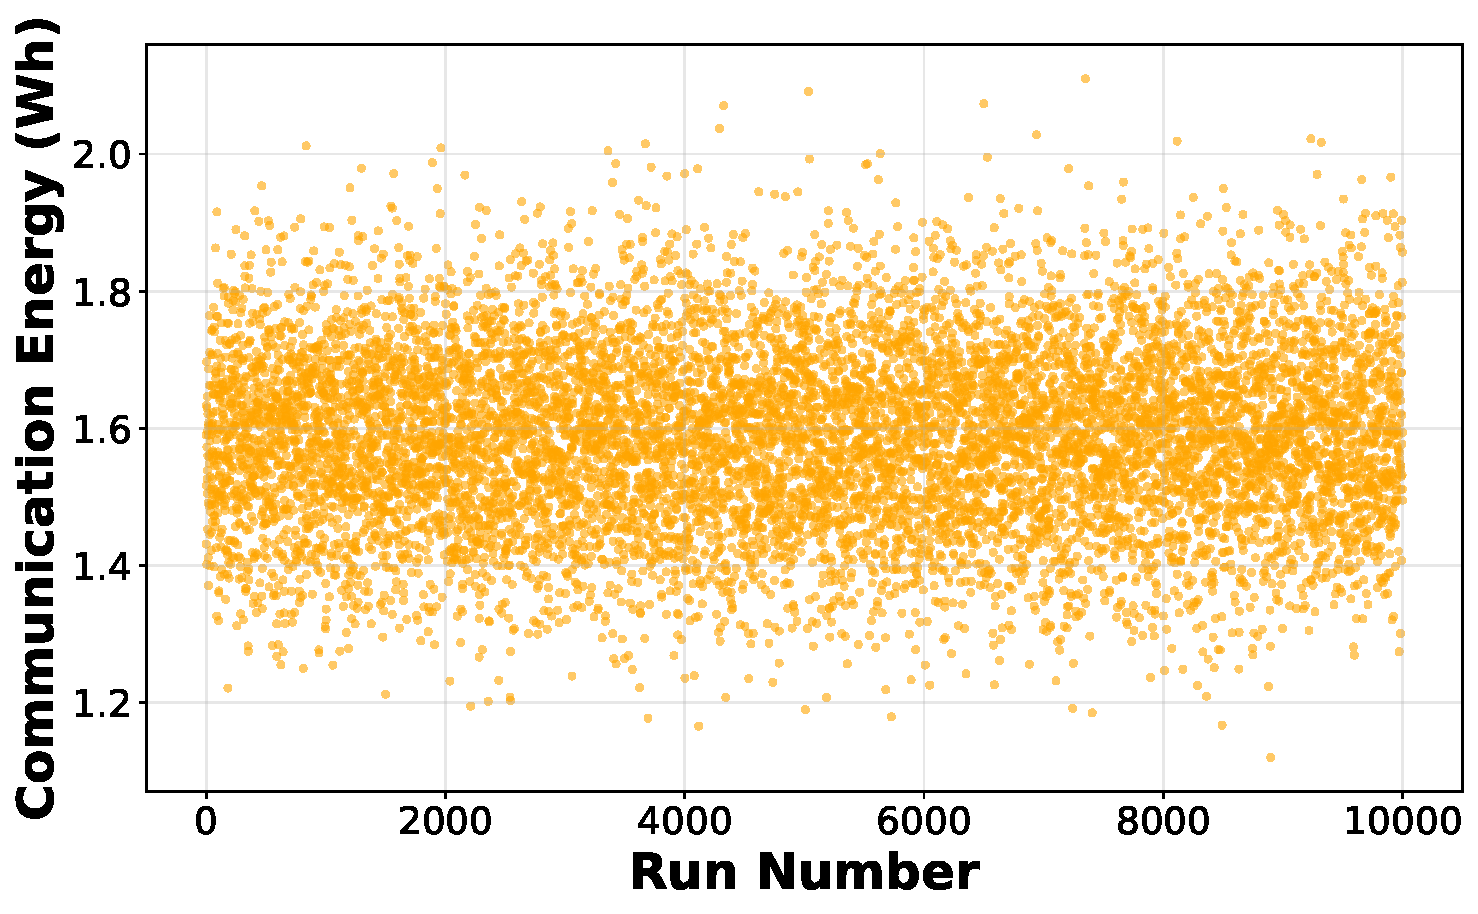
\includegraphics[width=0.48\textwidth]{figures/comm-energy-vs-run.pdf}
 %   \caption{Communication energy consumption for 10,000 Vicuna-7b tensor-parallel inference runs (128 output tokens) on 4 NVIDIA A6000 GPUs.}
  %  \label{fig:energy-variance}
%\end{figure}

%\noindent\textbf{Non-determinism.}
%\aruna{If we remove the figure, will this whole non-determinism piece go away? or do we still something about the non-determinism}
%Beyond this measurement complexity, tensor parallelism specifically introduces additional challenges with \be{synchronization} across GPUs as the ReduceScatter/AllGather phase is interleaved with layer computation for high efficiency.
%This introduces additional complications due \be{synchronization induced non-determinism} %that directly perturbs communication energy across runs.
%GPUs may lag/lead each other \be{non-deterministically} due to compute-time variation (e.g., memory-access and caching effects, hardware scheduling), creating \emph{idle-but-powered} intervals whose duration depends on runtime contention and race conditions. 
%Consequently, the time spent and the energy consumed in the communication phases can change even under \emph{identical} inputs and configurations.
%As shown in Figure~\ref{fig:energy-variance}, significant variation is observed in the measured communication energy when the same tensor-parallel inference (Vicuna-7b, in this case) is executed multiple times; see Section~\ref{ss:esetup} for experimental setup details.
%This creates \emph{idle-but-powered} intervals whose duration depends on runtime contention and race conditions. 
%This makes energy prediction more challenging. % complicating both isolating ``pure transfer'' energy from waiting energy and predicting a stable communication-energy contribution rather than a single deterministic trace.


% LLM energy consumption under parallel inference is driven by not only the computation cost, but also the \be{inter-GPU communication costs}. 
% This matters because communication can be a large fraction of total energy: Figure~\ref{fig:all_reduce_energy} shows that, for tensor-parallel runs, collective communication (e.g., AllReduce) contributes a substantial portion of end-to-end energy across model families and GPU counts (e.g., 14.2\%--35.1\% for Vicuna as model and GPU count scale). 
% \review{
% Predictors that extrapolate energy to multi-GPU settings solely from compute (or from per-rank tensor operations) systematically miss this component and can incur large errors.
% \textbf{Compute energy itself is non-trivial to model}, since it depends on how kernels exercise GPU resources (SM activity, memory intensity, and power-state behavior) across heterogeneous LLM modules.
% Prior work often sidesteps this by using \emph{coarse power measurements} (e.g., NVML board power sampled over time) or workload-level estimators (e.g., Strubell et al.’s energy-as-power$\times$time style accounting), and systems such as IrEne build learned predictors from profiled execution statistics.
% However, these approaches are typically \emph{coarse-grained and single-GPU oriented}, and they do not directly support accurate \emph{module-level} attribution under overlapping compute/communication in multi-GPU inference.
% }
% The severity and predictability of communication overhead differs across parallelism strategies.
% Under data parallelism, the replicas work independently,  
% except for the collation of output from each replica in the AllGather phase; as such, the additional energy of this phase needs to be accounted for. 
% %The AllGather phase is largely deterministic, so predicting the energy consumption under data parallel inference is feasible. 
% For pipeline parallelism, we have to track the energy consumption when data is sent from one stage to the other, in addition to the local computation. These data transfers happen in sync with each stage's computations and the timing can vary depending on sequence length and network speeds.

% Tensor parallelism is the most challenging of the three cases because synchronization across GPUs (e.g., ReduceScatter/AllGather) is interleaved with layer computation for high efficiency. This leads to two main challenges: 

% \noindent (i) \be{Non-determinism} in GPU wait times as GPUs often lag/lead each other in compute operations (due to variations in memory access, caching effects, hardware scheduling) during the synchronization phase. 
% From a measurement standpoint, this causes difficulty in isolating AllReduce energy as it requires distinguishing between the non-deterministic waiting phase (where GPUs are idle) and the network transfer phase.

% \noindent (ii) \be{Fine-grained energy accounting} is challenging as AllReduce overlaps computation and network transfer. 
% From a prediction standpoint, this requires isolating the different sources of energy consumption and accounting for them. 
% This is not an issue in pipeline and data parallelism as GPU communication and computation are not synchronized. 
% \review{
% Finally, \sys{} must also generalize across heterogeneous LLM variants, architectures, and deployment configurations, since changes in block structure (e.g., attention/MLP variants) and parallelization degree alter tensor shapes and collective-communication patterns, making predictors calibrated on one model/config unreliable on another~\cite{ultima}.
% }
%\smallskip\noindent{\textbf{Challenges: Communication energy in parallel inference.}}
%Energy consumption under parallel inference is shaped not only by local computation but also by inter-GPU \emph{communication} and the synchronization it induces. 
%}
